\documentclass{article}%
\usepackage[T1]{fontenc}%
\usepackage[utf8]{inputenc}%
\usepackage{lmodern}%
\usepackage{textcomp}%
\usepackage{lastpage}%
\usepackage[head=40pt,margin=0.5in,bottom=0.6in]{geometry}%
\usepackage{graphicx}%
%
\title{\textbf{Juventus derrota al Napoli y amplía su ventaja en la Serie A}}%
\author{AP}%
\date{03/03/2019}%
%
\begin{document}%
\normalsize%
\maketitle%
\textbf{URL: }%
http://www.eluniversal.com/deportes/34706/juventus{-}derrota{-}al{-}napoli{-}y{-}amplia{-}su{-}ventaja{-}en{-}la{-}serie{-}a\newline%
%
\textbf{Periodico: }%
EU, %
ID: %
34706, %
Seccion: %
deportes\newline%
%
\textbf{Palabras Claves: }%
NO\_TIENE\newline%
%
\textbf{Derecho: }%
2.1%
, Otros Derechos: %
\newline%
%
\textbf{\textit{La vecchia signora venció a los napolitanos 2{-}1 y sumó tres puntos para continuar su aparente marcha imparable rumbo al octavo título consecutivo en el campeonato italiano}}%
\newline%
\newline%
%
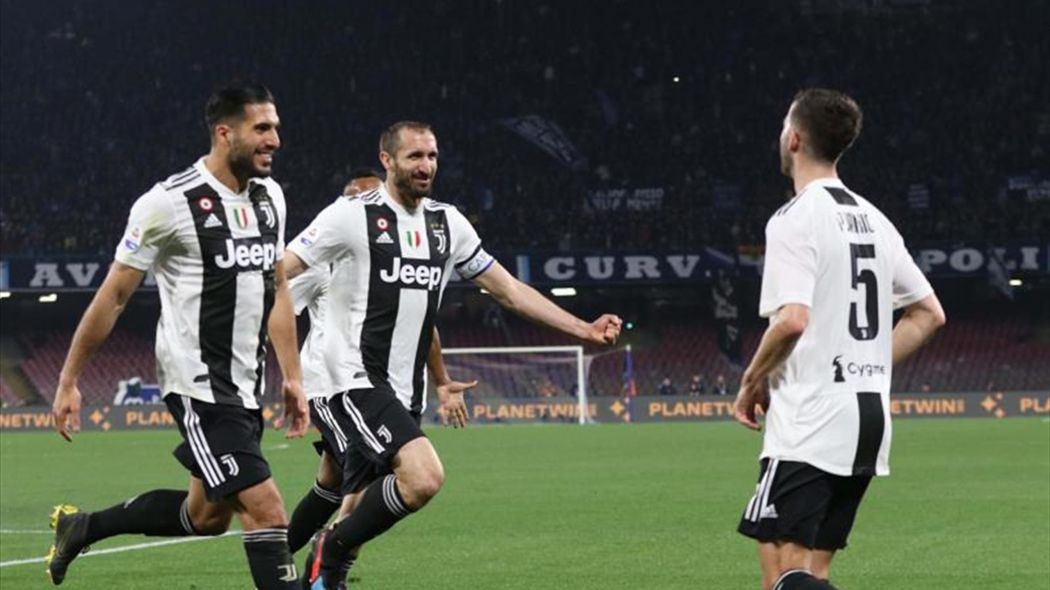
\includegraphics[width=300px]{EU_34706.jpg}%
\newline%
%
Roma.{-} Dos tarjetas rojas y un penalti fallado sobre el final formaron parte del libreto de un duelo dominical dramático en el estadio San Paolo, donde Juventus venció 2{-}1 al Napoli para continuar su aparente marcha imparable rumbo a un octavo título consecutivo de la Serie A.%
\newline%
%
Juventus parecía estar de paseo. Se fue al medio tiempo arriba por 2{-}0 y con un hombre más luego de la expulsión del portero del Napoli, Alex Meret, por una falta sobre Cristiano Ronaldo.%
\newline%
%
Pero Miralem Pjanic, autor del primer gol, fue también expulsado al inicio de la segunda mitad y José Callejón acercó al Napoli, sublíder de la clasificación.%
\newline%
%
Lorenzo Insigne estrelló un penalti en el poste a seis minutos del final, y la Juventus amplió su ventaja a 16 puntos en la Serie A.%
\newline%
%
El duelo cambió a los 28 minutos cuando Cristiano interceptó un mal pase de Kevin Malcuit y fue derribado al borde del área ante la salida de Meret.%
\newline%
%
Aunque fue debatible si Meret tocó al astro portugués, el árbitro Gianluca Rocchi mostró la tarjeta roja directa al portero del Napoli por su imprudencia para detener una oportunidad clara de gol.%
\newline%
%
Pjanic envió a las redes el tiro libre resultante de la infracción y Emre Can amplió la ventaja de la Juve 11 minutos después con un cabezazo a corta distancia.%
\newline%
%
Napoli encontró el camino para meterse de nuevo en el encuentro cuando Pjanic recibió la segunda amonestación por una mano a los dos minutos de la segunda mitad.%
\newline%
%
Los locales redujeron la distancia a los 61 cuando Callejón adelantó a los defensas de la Juventus para tocar un centro de Insigne.%
\newline%
%
Napoli se volcó sobre la portería de la Juventus y creyó encontrar su recompensa cuando se marcó el penal por una mano de Alex Sandro, pero el tiro de Insigne rebotó en el poste.%
\newline%
%
\end{document}